\documentclass[]{article}
\usepackage{lmodern}
\usepackage{amssymb,amsmath}
\usepackage{ifxetex,ifluatex}
\usepackage{fixltx2e} % provides \textsubscript
\ifnum 0\ifxetex 1\fi\ifluatex 1\fi=0 % if pdftex
  \usepackage[T1]{fontenc}
  \usepackage[utf8]{inputenc}
\else % if luatex or xelatex
  \ifxetex
    \usepackage{mathspec}
  \else
    \usepackage{fontspec}
  \fi
  \defaultfontfeatures{Ligatures=TeX,Scale=MatchLowercase}
\fi
% use upquote if available, for straight quotes in verbatim environments
\IfFileExists{upquote.sty}{\usepackage{upquote}}{}
% use microtype if available
\IfFileExists{microtype.sty}{%
\usepackage[]{microtype}
\UseMicrotypeSet[protrusion]{basicmath} % disable protrusion for tt fonts
}{}
\PassOptionsToPackage{hyphens}{url} % url is loaded by hyperref
\usepackage[unicode=true]{hyperref}
\hypersetup{
            pdftitle={Branching ratios in LiDAR scanned trees},
            pdfborder={0 0 0},
            breaklinks=true}
\urlstyle{same}  % don't use monospace font for urls
\usepackage[margin=1in]{geometry}
\usepackage{graphicx,grffile}
\makeatletter
\def\maxwidth{\ifdim\Gin@nat@width>\linewidth\linewidth\else\Gin@nat@width\fi}
\def\maxheight{\ifdim\Gin@nat@height>\textheight\textheight\else\Gin@nat@height\fi}
\makeatother
% Scale images if necessary, so that they will not overflow the page
% margins by default, and it is still possible to overwrite the defaults
% using explicit options in \includegraphics[width, height, ...]{}
\setkeys{Gin}{width=\maxwidth,height=\maxheight,keepaspectratio}
\IfFileExists{parskip.sty}{%
\usepackage{parskip}
}{% else
\setlength{\parindent}{0pt}
\setlength{\parskip}{6pt plus 2pt minus 1pt}
}
\setlength{\emergencystretch}{3em}  % prevent overfull lines
\providecommand{\tightlist}{%
  \setlength{\itemsep}{0pt}\setlength{\parskip}{0pt}}
\setcounter{secnumdepth}{0}
% Redefines (sub)paragraphs to behave more like sections
\ifx\paragraph\undefined\else
\let\oldparagraph\paragraph
\renewcommand{\paragraph}[1]{\oldparagraph{#1}\mbox{}}
\fi
\ifx\subparagraph\undefined\else
\let\oldsubparagraph\subparagraph
\renewcommand{\subparagraph}[1]{\oldsubparagraph{#1}\mbox{}}
\fi

% set default figure placement to htbp
\makeatletter
\def\fps@figure{htbp}
\makeatother


\title{Branching ratios in LiDAR scanned trees}
\author{}
\date{\vspace{-2.5em}}

\begin{document}
\maketitle

In the context of the WBE framework, the parameter \(n\) describes the
branching ratio. This parameter, also called the furcation number,
describes how volume is partitioned as vascular networks ramify down to
smaller and smaller size classes. One physiological interpretation is
that \(n\) is an integer, leading to a convenient representation of the
vascular network hierarchy

\begin{equation}
n_{k} = nn_{k+1} 
\end{equation}

where \(n_{k}\) is the number of vascular tubes at level \(k\). Thus,
the branching ratio is the source of self-similarity in WBE networks and
defines other geometric self-similarities in the form of branching
traits. Previous iterations of the WBE model have assumed that
\(n = 2\), which is the case of a perfectly symmetrical bifurcating
network. Most trees in nature appear to bifurcate regularly (as opposed
to trifurcation, etc.), but the branching ratio has posed an obstacle to
asymmetrical formulations of WBE by helping enforce the equal
distribution of parent volume/mass between child branches.

Our goal here is to explore the definition of the branching ratio, its
relationship with other quantities in vascular networks, and quantify
these within LiDAR scanned trees. One import expression states the
number of terminal tips of a network in terms of the branching ratio and
the maximum number of ramifications, or branching generations \(N\)
within a tree

\begin{equation} \label{eq:2}  
n_{N} = n^{N}
\end{equation}

The quantities \(n_{N}\) and \(N\) are directly available from LiDAR
scans before invoking any assumptions from WBE. From there, we can
compute the branching ratio for each subtree by rearranging \ref{eq:2}
as

\begin{equation} 
n = n_{N}^{1/N}
\end{equation}

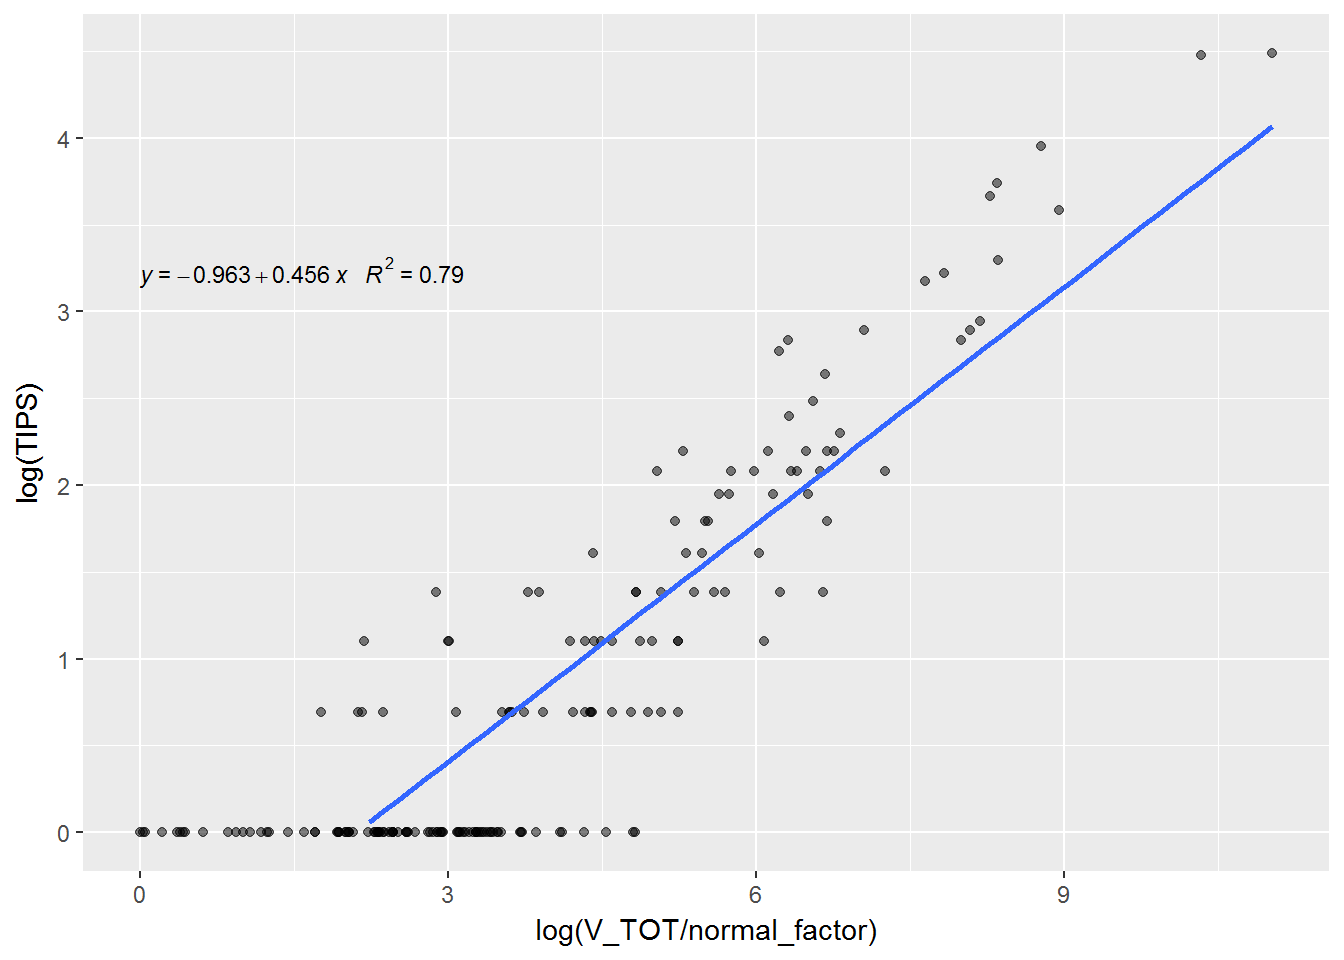
\includegraphics{branching_ratio_files/figure-latex/unnamed-chunk-1-1.pdf}

This method shows branching ratios universally below \(n=2\), which
would indicate that trees generally lack the number of terminal tip
elements predicted by the WBE framework, which we've already seen is an
important source of asymmetry in these data. An alternative view of the
branching ratio parameter is that it is a tree-level parameter, which
generally relates the number of terminal tips of a tree \(n_{N}\) to the
total depth of the tree (\(N\)) in the same way as in \ref{eq:2}. In
this case, we calculate \(n\) as a regression of terminal tips against
the depth of each subtree within a single network:

\begin{equation} \label{eq:3}  
log(n_{N}) / N = n
\end{equation}

\includegraphics{branching_ratio_files/figure-latex/unnamed-chunk-2-1.pdf}

This approach yields even lower branching ratios, universally \(n < 1\)
in this case. Interestingly, we can recover branching ratios in the
neighborhood of the method given by \ref{eq:2} by replacing the number
of terminal tips \$n\_\{N\} in \ref{eq:3} with the volume of terminal
tips \(V_{N}\):

\includegraphics{branching_ratio_files/figure-latex/unnamed-chunk-3-1.pdf}

Clearly we must reckon with branching ratios less than the idealized
\(n = 2\) case. Next, we should try to observe the effect of variation
in the furcation ratio on our predictions for metabolic scaling.

We should expect our branch scaling parameters to exhibit scaling ratios
closer to 1 as the branching ratio approaches 1. Branching ratios at or
below 1 would not intuitively correspond to bifurcation in the network,
instead approximating a linear network of equivalent (or progressively
larger) cylinders. We can ask whether this \emph{a priori} knowledge of
branching ratios should affect our predictions for the average values of
branching traits across trees in the dataset. These include the
following parameters for the scaling of radius and length across
branching generations:

\[\beta = n^{1/2},      \gamma = n^{1/3}\]

The following plot shows predicted and observed branching ratios as a
function of the branching ratio \(n\). We measure the branching ratio
for each tree following the method in \ref{eq:3}:
\includegraphics{branching_ratio_files/figure-latex/unnamed-chunk-4-1.pdf}

The branching ratio also independently affects the formula for the
metabolic scaling exponent:

\begin{equation} \label{eq:4}  
-\frac{log(n)}{log(\beta^{2}\gamma)} = \theta
\end{equation}

\includegraphics{branching_ratio_files/figure-latex/unnamed-chunk-5-1.pdf}
This plot shows that a reduction in the scaling ratio (\(n < 2\)) will
not move predictions for metabolic scaling closer to 3/4. It would move
theta, beta and gamma being equal, away from the optimal contour.
However, as we have seen, changing the branching ratio also changes our
predictions for scaling ratios. Therefore, the joint effects of \(n\) on
\(\beta, \gamma, and \theta\) are difficult to understand.

A major issue is that the single parameter \(n\) represents the average
behavior of child branches, which may behave in vastly different ways
according to the asymmetrical branching rules. This is evident from the
fact that, for values of \(n < 2\), we expect to observe larger scaling
parameters (closer to 1, where parent and child branches are identical).
Instead, our dataset of natural, asymmetrical trees exhibits scale
factors (especially length scaling factors) lower than those predicted
by the WBE framework. This is partially compensated for by asymmetrical
scale factors, but these newer factors lack an explicit definition in
terms of any generalized branching ratio, instead depending on cases
where \(n = 2\).

\end{document}
